\documentclass[twocolumn,superscriptaddress,aps]{revtex4-1}

\usepackage[utf8]{inputenc}

\usepackage{amsfonts}
\usepackage{amssymb}
\usepackage{amsmath}
\usepackage{amsthm}

\usepackage{bm}
\usepackage{cancel}
\usepackage{bbold}
\usepackage{slashed}
\usepackage{graphicx}
\usepackage{color}
\usepackage{hyperref}
\usepackage{algorithm}
\usepackage{algpseudocode}
\usepackage{tikz}

\newcommand{\glnote}[1]{\textcolor{red}{[GL: #1]}}

\theoremstyle{plain}
\newtheorem{theorem}{Theorem}
\newtheorem{proposition}[theorem]{Proposition}

\begin{document}


% ==============================================================================

\title{\Large{Adversarial Training against Systematic Uncertainty}}
\vspace{1cm}
\author{\small{\bf Gilles Louppe}\thanks{\texttt{g.louppe@nyu.edu}}}
\affiliation{New York University}
\author{\small{\bf Michael Kagan}\thanks{\texttt{makagan@slac.stanford.edu}}}
\affiliation{SLAC National Accelerator Laboratory}
\author{\small{\bf Kyle Cranmer}\thanks{\texttt{kyle.cranmer@nyu.edu}}}
\affiliation{New York University}

\begin{abstract}

In high energy physics, systematic uncertainties represent our incomplete
knowledge in the theory of physical processes or in the properties of the
experimental detection apparatus. In effect, these uncertainties typically cause
variations in the conditional distributions of the data, thereby altering the
decisions and resulting efficacy of a classifier trained from it. To contain
this issue, we propose to repurpose adversarial training as a means to learn a
pivotal classifier which is invariant to variations of the nuisance parameters
describing the effects of systematic uncertainties. In particular, we show and
derive theoretical conditions under which classification optimality and
invariance with respect to systematics can be achieved, which we confirm
experimentally on a couple of illustrative examples. In machine learning, this
problem is closely related to those of domain adaptation and enforcing fairness
in classification. Following that line of work, the proposed method can be
regarded as generalization that also supports the continuous case, which can be
viewed as handling infinitely many domains or as enforcing fairness over
continuous features.

\end{abstract}

\maketitle


% ==============================================================================

\section{Introduction}

The discovery of new particles or physical phenomena in high energy physics
experiments, like those at the Large Hadron Collider, requires the observation
of statistically significant deviations from the predictions of the Standard
Model, the current model of the known fundamental particles and their
interactions.  Typically, discovery requires satisfying the \textit{5-sigma
rule}, whereby the deviation must be at least five standard deviations from
predictions, i.e. having a p-value of $p \lesssim 3 \times 10^{-7}$. The
evaluation of the statistical significance must not only account for statistical
uncertainties due to random fluctuations, but also for
systematic uncertainties that represent our incomplete knowledge of the theory
of particle interactions or of the properties of the experimental detection
apparatus. Systematic uncertainties can alter the expected rate of signal and
background classes, e.g. their priors, as well as the distributions of features.
As such, the signal class true-positive rate and the background class
false-positive rate of a classifier can change with variations in the systematic
uncertainty thereby decreasing the sensitivity of an analysis. In this paper, we
present a new strategy for training a classifier, based on adversarial
training~\citep{goodfellow2014generative}, which aims at building a classifier
whose decision function is invariant under variations due to systematic
uncertainties.  In this way, uncertainties on predictions from simulations will
have a reduced impact when computing the significance of potential deviations
after application of the discriminant model and thereby increase the sensitivity
of the analysis to signals from potential new physics sources.

Given data $X$ and associated labels $Y$
taking values $y \in {\cal Y} = \{s,
b_{i=1...k} \}$ where $s$ is the signal class and $b_{i=1...k}$ are
the background classes, the probability density of the data
can be written as a mixture
\begin{equation}
p(X) = \pi_s p(X|Y=s) + \sum_{i=1}^{k} \pi_{b_i} p(X | Y=b_i),
\end{equation}
where $\pi_{y}$ represents the prior for the signal or a given
background, and $p(X|Y)$ is the conditional distribution of the data
for the signal or a given background. Systematic uncertainties can
affect this distribution in the following ways \citep{sinervo2003definition,bohm2010introduction}:
\begin{itemize}
\item Uncertainties on the priors $\pi_{y}$.  These arise from
  uncertainties on the rates we expect a given process to occur as
  predicted from theoretical calculations or from alternative
  measurements of the rate of a given class.

\item Uncertainties in the simulators of the physical interactions,
  giving rise to uncertainties on the distributions $p(X|Y)$.  These
  uncertainties are often determined by comparing the predictions of
  different simulations using differing models of the same physical
  process.

\item Uncertainties on the detection apparatus and its effect on the
  measurement of particle properties, giving rise to uncertainties on
  the distributions $p(X|Y)$.  For instance, this includes
  uncertainties on our knowledge of the mean and variance of the
  measured energy distribution of a particle.
\end{itemize}
In this paper, we will not address uncertainties of the first type
mentioned above (uncertainties on the priors).  Rather, we will focus
on mitigating the effect of systematic uncertainties that alter the
conditional distributions $p(X|Y)$. \glnote{Remove this comment?}

Systematic uncertainties are parameterized by nuisance parameters in the
statistical analysis of data (see e.g.,
\citep{bohm2010introduction,cowan2011asymptotic}).  Nuisance parameters often,
though not always, have a suitable prior coming from alternative measurements in
data.  For instance, the average measured energy of an electron in simulation
may be compared with those in data using a relatively pure sample of $Z$ boson
decays to electrons.  The average measured electron energy can not be measured
without uncertainty, and the measured uncertainty can be used in other analyses
to estimate the uncertainty deriving from our imperfect knowledge of the
electron's energy.  A nuisance parameter is assigned to the electron energy
uncertainty, which controls the variation of the electron energy in the
statistical analysis of data.  Nuisance parameters are typically, though not
always, constrained by a suitable prior, e.g. a Gaussian distribution with a
standard deviation equal to the measured uncertainty. \glnote{This paragraph
could be improved, it is not very clear what we want to say...}

\glnote{Add paper outline.}

% ==============================================================================

\section{Problem statement}
\label{sec:problem}

Let assume a probability space $(\Omega, {\cal F}, P)$, where $\Omega$ is a
sample space, ${\cal F}$ is a set of events and $P$ is a probability measure.
Let consider the multivariate random variables $X_z: \Omega \mapsto
\mathbb{R}^p$ and $Y: \Omega \mapsto {\cal Y}$, where $X_z$ denotes a dependence
of the functional $X$ on a nuisance parameter $Z$, whose values $z \in {\cal Z}$  define a
parameterized family of its systematic uncertainties. That is, $X_z$ and $Y$
induce together a joint probability distribution $p(X,Y|Z=z)$, where the
conditional denotes $X_z$. For training, let further assume a finite set $\{
x_i, y_i, z_i \}_{i=1}^N$ of realizations $X_{z_i}(\omega_i), Y(\omega_i)$, for
$\omega_i \in \Omega$ and known values $z_i$ of the nuisance parameter. Our goal
is to learn a score function $f(\cdot;\theta_f) : \mathbb{R}^p \mapsto {\cal S}$ of
parameters $\theta_f$ (e.g., a neural network-based probabilistic classifier) and minimizing  a loss ${\cal L}_f(\theta_f)$ (e.g.,
the cross-entropy). In addition, we require that $f(X_z ; \theta_f)$ should be
robust to the value $z$ of the nuisance parameter  -- which remains unknown at
test time. More specifically, we aim at building $f$ such that in the ideal case
\begin{equation}\label{eqn:criterion-true}
f(X_{z}(\omega) ; \theta_f) = f(X_{z^\prime}(\omega) ; \theta_f)
\end{equation} for all
samples $\omega \in \Omega$ and all $z, z^\prime$ pairs of values of the
nuisance parameter.

Since in general we do not have training tuples $(X_{z}(\omega),
X_{z^\prime}(\omega))$ (for the same unknown $\omega$), we propose instead to
solve the closely related problem of finding a predictive function $f$ such that
\begin{align}\label{eqn:criterion-measure}
    &P(\{ \omega | f(X_{z}(\omega) ; \theta_f) = s \} ) \nonumber \\
    &\indent = P( \{ \omega' | f(X_{z^\prime}(\omega') ; \theta_f) = s\})
\end{align}
for all values $s \in {\cal S}$ taken by the score function $f$. In words, we are looking for a predictive function $f$
which is a pivotal quantity \citep{degroot1986probability} with respect to the
nuisance parameter. That is, such that  the distribution of $f(X_z; \theta_f)$
is invariant with respect to the value $z$ of the nuisance. Note that a function
$f$ for which Eqn.~\ref{eqn:criterion-true} is true necessarily satisfies
Eqn.~\ref{eqn:criterion-measure}. In general, the converse is however not true,
since the sets of samples $\{ \omega | f(X_{z}(\omega); \theta_f) = s \}$ and $\{
\omega' | f(X_{z^\prime}(\omega'); \theta_f) = s \}$ do not need to be the same
for the equality to hold. In order to simplify notations, and as only
Eqn.~\ref{eqn:criterion-measure} is of direct interest in this work, we denote
from here on the pivotal quantity criterion as
\begin{equation}\label{eqn:criterion}
    p(f(X ; \theta_f) = s | z ) = p(f(X ; \theta_f) = s | z^\prime )
\end{equation}
for all $z,z^\prime \in  {\cal Z}$ and all values $s \in {\cal S}$ of $f(X ; \theta_f)$.


% ==============================================================================

\section{Method}
\label{sec:method}

Joint training of adversarial networks was first proposed by \citep{goodfellow2014generative} as a
way to build a generative model capable of producing samples from random noise
$z$. More specifically, the authors pit a generative model $g:
\mathbb{R} \mapsto \mathbb{R}^p$ against an adversary classifier $d :
\mathbb{R}^p \mapsto [0, 1]$ whose antagonistic objective is to recognize
real data $X$ from generated data $g(Z)$. Both models $g$ and $d$ are trained
simultaneously, in such a way that $g$ learns to produce samples that are
difficult to identify by $d$, while $d$ incrementally adapts to changes in $g$.
At the equilibrium, $g$ models a distribution whose samples can be identified by
$d$ only by chance. That is, assuming enough capacity in $d$ and  $g$, the
distribution of $g(Z)$ eventually converges towards the real distribution
of $X$.

\tikzstyle{every node}=[font=\scriptsize]
\begin{figure*}
    \usetikzlibrary{arrows}
    \def\layersep{1cm}

    \begin{tikzpicture}[shorten >= 1pt, ->, node distance=\layersep,scale=.85]
    \tikzstyle{neuron} = [circle, minimum size=0.25cm, draw=black!30, line width=0.3mm, fill=white]

    % Classifier f
    \node at (2,0) {Classifier $f$};
    \draw (-1,-0.5) rectangle (4,-5.5);

    \path[->, shorten >= 0pt] (-2,-3) edge (-1,-3);
    \node[left] at (-2,-3) {$X$};

    \path[-o, shorten >= 0pt] (1.5,-6.5) edge (1.5,-5.5);
    \node[below] at (1.5,-6.5) {$\theta_f$};

    \path[->, shorten >= 0pt] (3.5,-3) edge (6.5,-3);
    \node[above] at (5.25,-3) {$f(X;\theta_f)$};

    \path[dashed,-] (5.25,-3) edge (5.25,-6.5);
    \node[below] at (5.25,-6.5) {${\cal L}_f(\theta_f)$};

    \foreach \name / \y in {1,...,3}
        \node[neuron] (f-I-\name) at (-0.5,-1-\y) {};

    \foreach \name / \y in {1,...,5}
        \node[neuron] (f-H1-\name) at (-0.5cm+\layersep,-\y cm) {};
    \foreach \name / \y in {1,...,5}
        \node[neuron] (f-H2-\name) at (-0.5cm+3*\layersep,-\y cm) {};

    \node[neuron] (f-O) at (-0.5cm+4*\layersep,-3cm) {};

    \foreach \source in {1,...,3}
        \foreach \dest in {1,...,5}
            \path[black!20] (f-I-\source) edge (f-H1-\dest);

    \foreach \source in {1,...,5}
        \path[black!30] (f-H2-\source) edge (f-O);

    \node[black!30] at (1.5,-3) {...};

    % Adversary r
    \node at (11.75,0) {Adversary $r$};
    \draw (6.5,-0.5) rectangle (11.5,-5.5);

    \node[above] at (12.75,-2) {$\gamma_1(f(X;\theta_f);\theta_r)$};
    \path[-o, shorten >= 0pt] (11,-2.0) edge (14,-2.0);
    \node[above] at (12.75,-3) {$\gamma_2(f(X;\theta_f);\theta_r)$};
    \path[-o, shorten >= 0pt] (11,-3) edge (14,-3);
    \node[above] at (12.75,-4) {$\dots$};
    \path[-o, shorten >= 0pt] (11,-4) edge (14,-4);

    \path[-o, shorten >= 0pt] (9,-6.5) edge (9,-5.5);
    \node[below] at (9,-6.5) {$\theta_r$};

    \foreach \name / \y in {1,...,1}
        \node[neuron] (r-I-\name) at (7,-2-\y) {};

    \foreach \name / \y in {1,...,5}
        \node[neuron] (r-H1-\name) at (7cm+\layersep,-\y cm) {};
    \foreach \name / \y in {1,...,5}
        \node[neuron] (r-H2-\name) at (7cm+3*\layersep,-\y cm) {};

    \node[neuron] (r-O1) at (7cm+4*\layersep,-2cm) {};
    \node[neuron] (r-O2) at (7cm+4*\layersep,-3cm) {};
    \node[neuron] (r-O3) at (7cm+4*\layersep,-4cm) {};

    \foreach \source in {1,...,1}
        \foreach \dest in {1,...,5}
            \path[black!20] (r-I-\source) edge (r-H1-\dest);

    \foreach \source in {1,...,5}
        \path[black!30] (r-H2-\source) edge (r-O1);
    \foreach \source in {1,...,5}
        \path[black!30] (r-H2-\source) edge (r-O2);
    \foreach \source in {1,...,5}
        \path[black!30] (r-H2-\source) edge (r-O3);

    \node[black!30] at (9,-3) {...};

    \draw (14,-1.5) rectangle (17,-4.5);
    \path[->, shorten >= 0pt] (15.5,-0.5) edge (15.5,-1.5);
    \node[above] at (15.5,-0.5) {$Z$};
    \path[->, shorten >= 0pt] (15.5,-4.5) edge (15.5,-5.5);
    \node[below] at (15.5,-5.5) {$p_{\theta_r}(Z|f(X;\theta_f))$};
    \node at (15.5,-3) {${\cal P}(\gamma_1, \gamma_2, \dots)$};

    \draw[dashed,-] (15.5,-5) -| (12.75,-6.5);
    \node[below] at (12.75,-6.5) {${\cal L}_r(\theta_f, \theta_r)$};

    \end{tikzpicture}

    \caption{Architecture for the adversarial training of a binary classifier
    $f$ against a nuisance parameter $Z$. The adversary $r$ models the
    distribution $p(z|f(X;\theta_f)=s)$ of the nuisance as observed only through the output $f(X;\theta_f)$ of the classifier. By
    maximizing the antagonistic objective ${\cal L}_r(\theta_f, \theta_r)$ (as part of minimizing ${\cal L}_f(\theta_f) - \lambda {\cal L}_r(\theta_f, \theta_r)$), the classifier
    $f$ forces $p(z|f(X;\theta_f)=s)$ towards the prior $p(z)$, which happens
    when $f(X;\theta_f)$ is  independent of the nuisance parameter $Z$ and therefore pivotal.}

    \label{fig:architecture}
\end{figure*}

In this work, we repurpose adversarial networks as a means to constraint the
predictive model $f$ in order to satisfy Eqn.~\ref{eqn:criterion}. As
illustrated in Fig.~\ref{fig:architecture}, we pit $f$ against an adversary
model $r := p_{\theta_r}(z | f(X;\theta_f)=s)$ of parameters $\theta_r$ and
associated loss ${\cal L}_r(\theta_f, \theta_r)$. This model takes  as input
realizations $s$ of $f(X; \theta_f)$, for the current value $\theta_f$ of $f$
parameters, and produces as output a function $p_{\theta_r}(z | f(X;\theta_f)=s)$
modeling the posterior probability density that $z$ parameterizes the sample
observed as $s$.
Intuitively, if $p(f(X; \theta_f)=s|z)$ varies with $z$,
then the corresponding correlation can be captured by $r$. By contrast, if
$p(f(X; \theta_f)=s|z)$ is invariant with $z$, as we require, then $r$ should
perform poorly and be close to random guessing. Training $f$ such that it
additionally minimizes the performance of $r$ therefore acts as a regularization
towards Eqn.~\ref{eqn:criterion}.

If $Z$ takes discrete values, then $p_{\theta_r}$ can be represented e.g. as a
probabilistic classifier $\mathbb{R} \mapsto \mathbb{R}^{|{\cal Z|}}$ whose
output $j$ (for $j=1, \dots, |{\cal Z}|$) is the estimated probability mass
$p_{\theta_r}(z_j|f(X;\theta_f)=s)$. Similarly, if $Z$ takes continuous values and
if we assume some parameteric distribution ${\cal P}$ for $Z|f(X;\theta_f)=s$
(e.g., a mixture of gaussians, as modeled with a mixture
density network~\citep{bishop1994mixture}), then $p_{\theta_r}$ can be
represented e.g. as network whose output $j$ is the estimated value of the
corresponding parameter $\gamma_j$ of that distribution (e.g., the mean,
variance and mixing coefficients of its components). As in
\citep{nix1994estimating,bishop1994mixture}, the estimated probability density
$p_{\theta_r}(z|f(X;\theta_f)=s)$ can then be evaluated for any $z \in {\cal Z}$ and any score $s \in {\cal S}$.
As further explained in the next section, let us note that the adversary $r$ may
take any form, i.e. it does need to be a neural network, as long as it exposes a
differentiable function $p_{\theta_r}(z|f(X;\theta_f)=s)$ of sufficient capacity
to represent the true distribution.

As for generative adversarial networks, we propose to
train $f$ and $r$ simultaneously, which we carry out by considering
the value function
\begin{equation}
    E(\theta_f, \theta_r) = {\cal L}_f(\theta_f) - {\cal L}_r(\theta_f, \theta_r)
\end{equation}
that we optimize by finding the saddle point $(\smash{\hat\theta_f}, \smash{\hat\theta_r})$ such that
\begin{align}
    \smash{\hat\theta_f} &= \arg \min_{\theta_f} E(\theta_f, \smash{\hat\theta_r}), \label{eqn:min_thetaf} \\
    \smash{\hat\theta_r} &= \arg \max_{\theta_r} E(\smash{\hat\theta_f}, \theta_r) \label{eqn:max_thetar}.
\end{align}
Without loss of generality, the adversarial training procedure to obtain
$(\smash{\hat\theta_f}, \smash{\hat\theta_r})$ is formally presented in
Algorithm~\ref{alg:adversarial-training} in the case of a binary classifier $f :
\mathbb{R}^p \mapsto [0,1]$ modeling $p(Y=1|X)$. For reasons further explained
in Section~\ref{sec:theory}, ${\cal L}_f$ and ${\cal L}_r$  are respectively set to the
expected value of the
negative log-likelihood of $Y|X$ under $f$ and of $Z|f(X;\theta_f)$ under
$r$:
\begin{align}
    {\cal L}_f(\theta_f) &= \mathbb{E}_{x \sim X}  \mathbb{E}_{y \sim Y|x} [ -\log p_{\theta_f} (y|x) ], \\
    {\cal L}_r(\theta_f, \theta_r) &= \mathbb{E}_{s \sim f(X;\theta_f)}  \mathbb{E}_{z \sim Z|s} [-\log p_{\theta_r} (z|s)].
\end{align}
The optimization algorithm consists in using stochastic gradient descent
alternatively for solving Eqn.~\ref{eqn:min_thetaf} and \ref{eqn:max_thetar}.

\begin{figure*}
    \begin{minipage}{\linewidth}
    \begin{algorithm}[H]
    \caption{Adversarial training of a classifier $f$ against an adversary $r$.}

    \begin{flushleft}
        {\it Inputs:} training data $\{ x_i, y_i, z_i \}_{i=1}^N$;\\
        {\it Outputs:} $\smash{\hat\theta_f}, \smash{\hat\theta_r}$;\\
        {\it Hyper-parameters:} Number $T$ of training iterations,
                                Number $K$ of gradient steps to update $r$.
    \end{flushleft}

    \label{alg:adversarial-training}
    \begin{algorithmic}[1]
        \For{$t=1$ to $T$}
            \For{$k=1$ to $K$} \Comment{Update $r$}
                \State{Sample minibatch $\{x_m, z_m, s_m = f(x_m;\theta_f) \}_{m=1}^M$} of size $M$;
                \State{With $\theta_f$ fixed, update $r$ by ascending its stochastic gradient $\nabla_{\theta_r} E(\theta_f, \theta_r) :=$
                $$\nabla_{\theta_r} \sum_{m=1}^M \log p_{\theta_r}(z_m|s_m)  ;$$}
            \EndFor
            \State{Sample minibatch $\{x_m, y_m, z_m, s_m = f(x_m;\theta_f)  \}_{m=1}^M$} of size $M$; \Comment{Update $f$}
            \State{With $\theta_r$ fixed, update $f$ by descending its stochastic gradient $\nabla_{\theta_f} E(\theta_f, \theta_r) :=$
            $$\nabla_{\theta_f}  \sum_{m=1}^M \left[ -\log p_{\theta_f}(y_m|x_m)  +\log p_{\theta_r}(z_m|s_m)  \right],$$
            \indent where $p_{\theta_f}(y_m|x_m)$ denotes $1(y_m=0)(1-s_m) + 1(y_m=1)s_m$;}
        \EndFor
    \end{algorithmic}
    \end{algorithm}
    \end{minipage}
\end{figure*}


% ==============================================================================

\section{Theoretical results}
\label{sec:theory}

In this section, we show that in the setting of
Algorithm~\ref{alg:adversarial-training} where ${\cal L}_f$ and ${\cal L}_r$ are
respectively set to expected value of the negative log-likelihood of $Y|X$ under
$f$ and of $Z|f(X;\theta_f)$ under $r$, the procedure converges to a classifier
$f$ which is a pivotal quantity in the sense of Eqn.~\ref{eqn:criterion}.

In this setting, the nuisance parameter $Z$ is considered as a random variable
of prior $p(z)$ (for $z \in {\cal Z}$), and our goal is to find a function
$f(\cdot;\theta_f)$ such that $f(X;\theta_f)$ and $Z$ are independent random
variables.   Importantly, classification of $Y$ with respect to $X$ is
considered in the context where $Z$ is marginalized out, which means that the
classifier minimizing ${\cal L}_f$ is optimal with respect to $Y|X$, but not
necessarily with $Y|X,Z$ (unless $Z$ is made explicit and is included among the
input variables in $X$). Results hold for a nuisance parameter $Z$ taking either
categorical or continuous values. By abuse of notation, $H(Z)$ denotes the
differential entropy in this latter case. Finally, the  proposition below is
derived in a non-parametric setting, by assuming that both $f$ and $r$ have
enough capacity.

\begin{proposition}\label{prop:2}
If there exists a saddle point $(\smash{\hat\theta}_f, \smash{\hat\theta}_r)$
for Eqn.~\ref{eqn:min_thetaf} and \ref{eqn:max_thetar} such that
$E(\hat\theta_f, \hat\theta_r) = H({Y|X}) - H(Z)$, then
$f(\cdot;\smash{\hat\theta}_f)$ is both an optimal classifier and a pivotal
quantity.
\end{proposition}

\begin{proof}

For fixed $\theta_f$, the adversary $r$ is optimal at $$\hat\theta_r = \arg
\max_{\theta_r} E(\theta_f, \theta_r)  = \arg \min_{\theta_r} {\cal
L}_r(\theta_f, \theta_r),$$ in which case $p_{\hat\theta_r}(z|f(X;\theta_f)=s) =
p(z|f(X;\theta_f)=s)$ for all $z$ and all $s$, and ${\cal L}_r$ reduces to the expected entropy
$\mathbb{E}_{s \sim f(X;\theta_f)} [ H({Z|f(X;\theta_f)=s}) ]$ of the conditional distribution of the nuisance.
This expectation is nothing else than the conditional entropy of the random variables
$Z$ and $f(X;\theta_f)$ and can be written as $H(Z|f(X;\theta_f))$.
Accordingly, the
value function $E$ can be restated as a function depending on $\theta_f$ only: $$E'(\theta_f) = {\cal
L}_f(\theta_f) -  H({Z|f(X;\theta_f)}).$$  In particular, we have the lower
bound $$H({Y|X}) - H(Z) \leq {\cal L}_f(\theta_f) - H({Z|f(X;\theta_f)})$$
where the equality holds at $\smash{\hat\theta}_f = \arg \min_{\theta_f}
E'(\theta_f)$  when:
\begin{itemize}
    \item $\smash{\hat\theta}_f$ minimizes the negative log-likelihood of $Y|X$ under $f$,
    which happens when $\smash{\hat\theta}_f$ are the parameters
    of an optimal classifier. In this case, ${\cal L}_f$ reduces to its
    minimum value $H({Y|X})$.

    \item $\smash{\hat\theta}_f$ maximizes the conditional entropy
    $H({Z|f(X;\theta_f)})$ since $H(Z|f(X;\theta)) \leq H(Z)$. Note that this
    latter inequality holds for both the discrete and the differential definitions of entropy.
\end{itemize}
When the lower bound is active, we have $H(Z|f(X;\theta_f)) = H(Z)$
because of the second condition, which happens exactly when $Z$ and $f(X;\theta_f)$
are independent variables. In other words,  the
optimal classifier $f(\cdot;\smash{\hat\theta}_f)$ is also a pivotal
quantity.

\end{proof}

Proposition~\ref{prop:2} suggests that if at each step of
Algorithm~\ref{alg:adversarial-training} the adversary $r$ is allowed to reach
its optimum given $f$ (e.g., by setting $K$ sufficiently high) and if $f$ is
updated to improve ${\cal L}_f(\theta_f) -  H({Z|f(X;\theta_f)})$, then $f$
should converge to a classifier which is both optimal and pivotal, provided such
a classifier exists. A formal proof of convergence of the alternating
stochastic gradient descent procedure of
Algorithm~\ref{alg:adversarial-training} remains however to be proven.

On many practical problems, let us note that such a classifier may
not exist because the nuisance parameter directly shapes the decision boundary.
In this case, the lower bound $ H({Y|X}) - H(Z) < {\cal L}_f(\theta_f) - H({Z|f(X;\theta_f)})$ is strict: $f$ can either be an optimal classifier or a
pivotal quantity, but not both simultaneously. In this situation, it is natural
to rewrite the value function $E$  as
\begin{equation}\label{eqn:vf-lambda}
    E_\lambda(\theta_f, \theta_r) = {\cal L}_f(\theta_f) - \lambda {\cal L}_r(\theta_f, \theta_r),
\end{equation}
where $\lambda \geq 0$ is a hyper-parameter controlling the trade-off between
the performance of $f$ and its independence with respect to the nuisance
parameter. Setting $\lambda$ to a large value will preferably enforces $f$ to
be pivotal while setting $\lambda$ close to $0$ will rather constraint $f$ to be
optimal.

Interestingly, let us finally emphasize that these results hold using only the (1D) output $s$
of $f(\cdot;\theta_f)$ (in the case of binary classification) as input to the adversary. We
could similarly enforce an intermediate representation of the data to be
pivotal, e.g. as in \citep{ganin2014unsupervised}, but this is in fact not
necessary.


% ==============================================================================

\section{Experiments}

\subsection{Toy example}
\label{sec:toy}

\begin{figure*}
    \begin{center}
        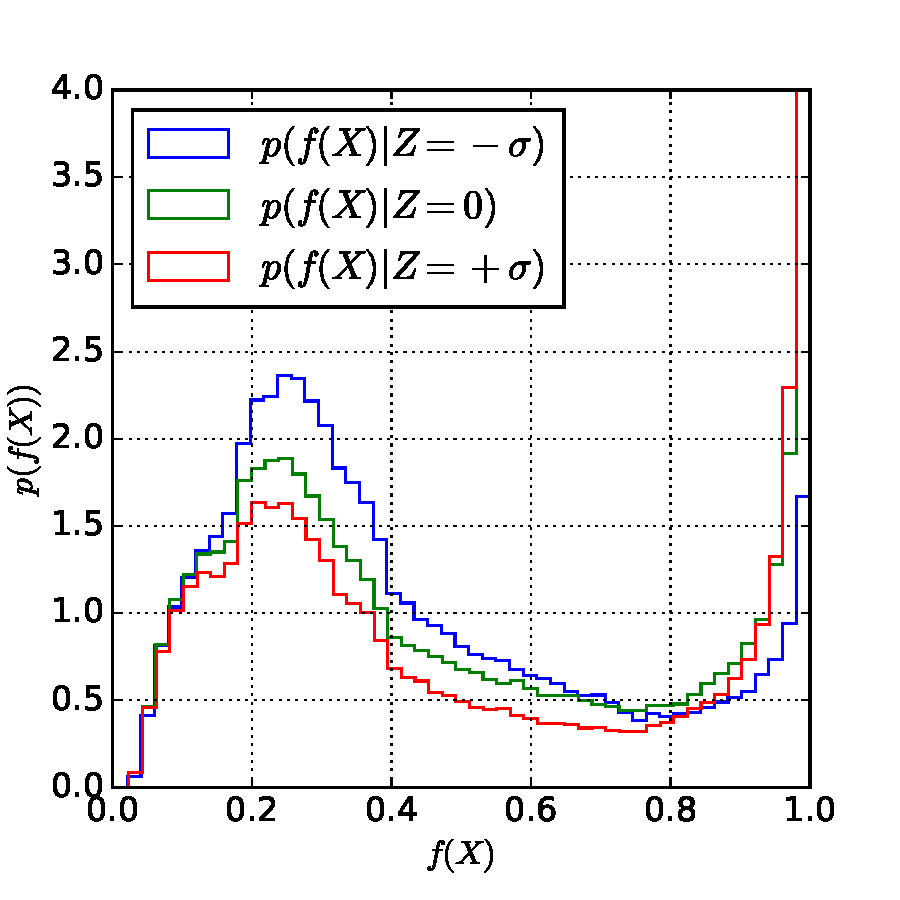
\includegraphics[width=0.48\textwidth]{figures/f-plain.pdf}
        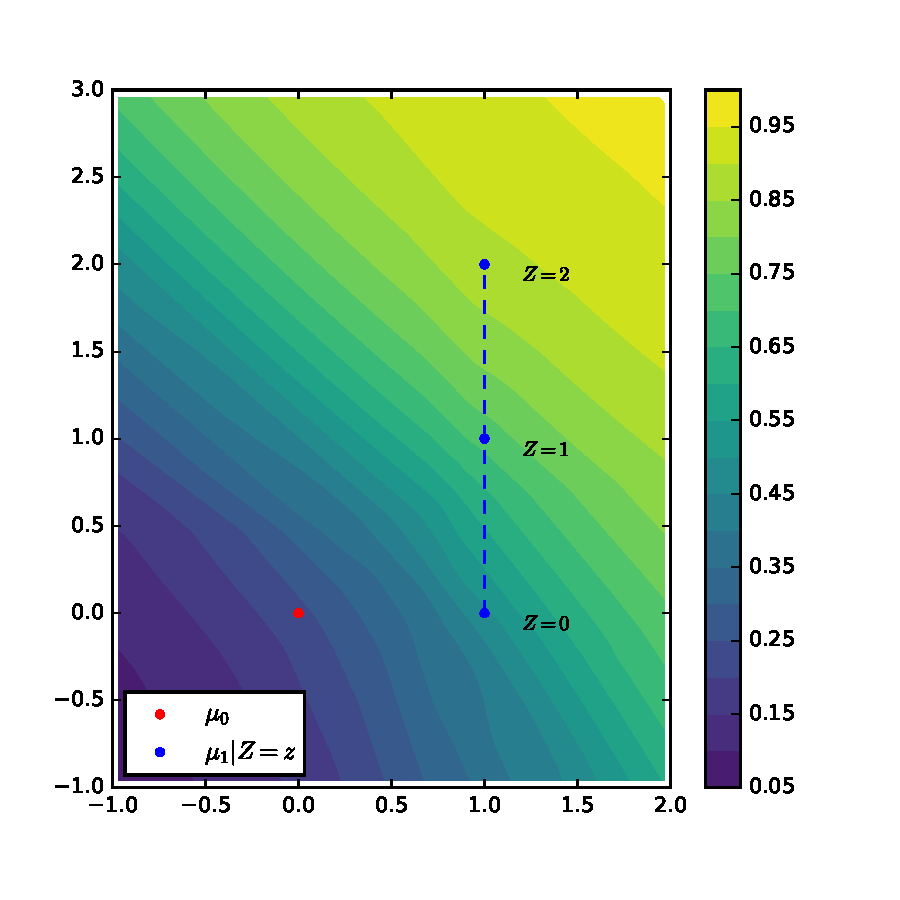
\includegraphics[width=0.48\textwidth]{figures/surface-plain.pdf}\\
        \vspace{-0.8cm}
        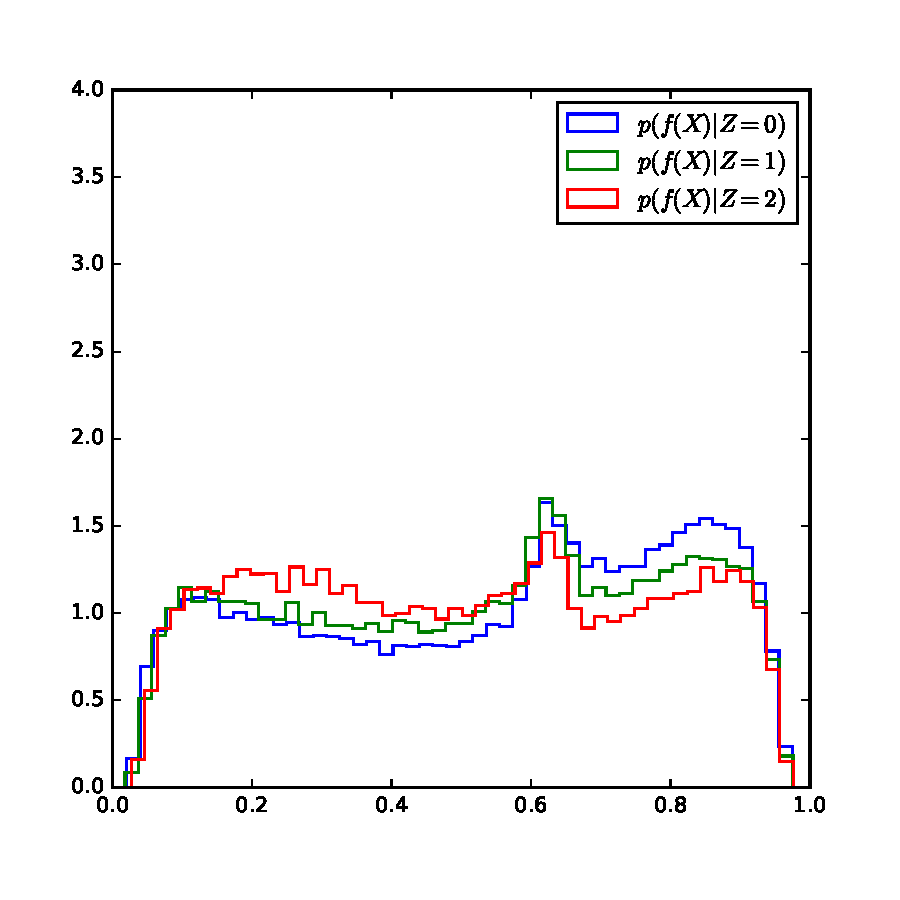
\includegraphics[width=0.48\textwidth]{figures/f-adversary.pdf}
        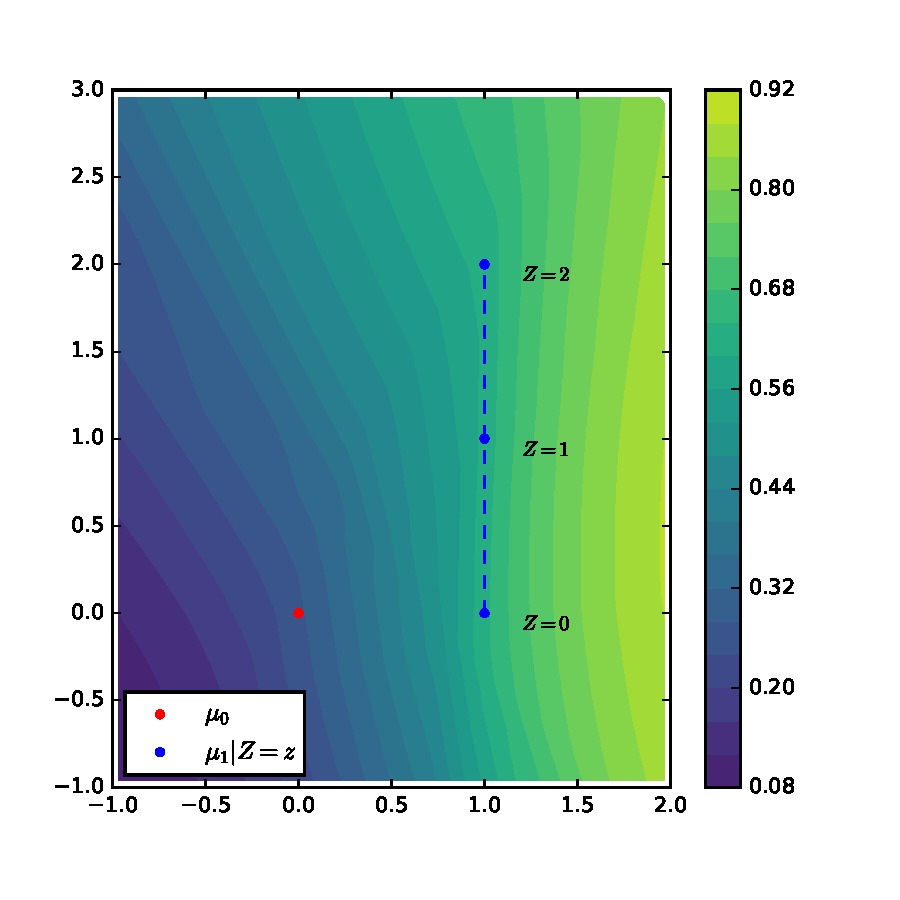
\includegraphics[width=0.48\textwidth]{figures/surface-adversary.pdf}
    \end{center}
    \vspace{-1cm}
    \caption{Toy example.
    (Upper left) Conditional probability densities of the decision scores at $Z=-\sigma, 0, \sigma$
       when $f$ is built without adversarial training. The resulting densities
       are clearly dependent on the continuous parameter $Z$, indicating that $f$ is not pivotal.
    (Upper right) The corresponding decision surface, highlighting
       the fact that samples are easier to classify for values of $Z$ above to $\sigma$,
       hence partially explaining the dependency.
    (Lower left) Conditional probability densities of the decision scores at $Z=-\sigma, 0, \sigma$ when $f$ is
       built with adversarial training, as outlined in Section~\ref{sec:method}.
       The resulting densities are now almost identical to each other, indicating only a
       small dependency on $Z$.
    (Lower right) The corresponding decision surface, illustrating how adversarial
       training bends the decision function vertically to erase the dependency on $Z$.
    }
    \label{fig:toy}
\end{figure*}

\begin{figure}
    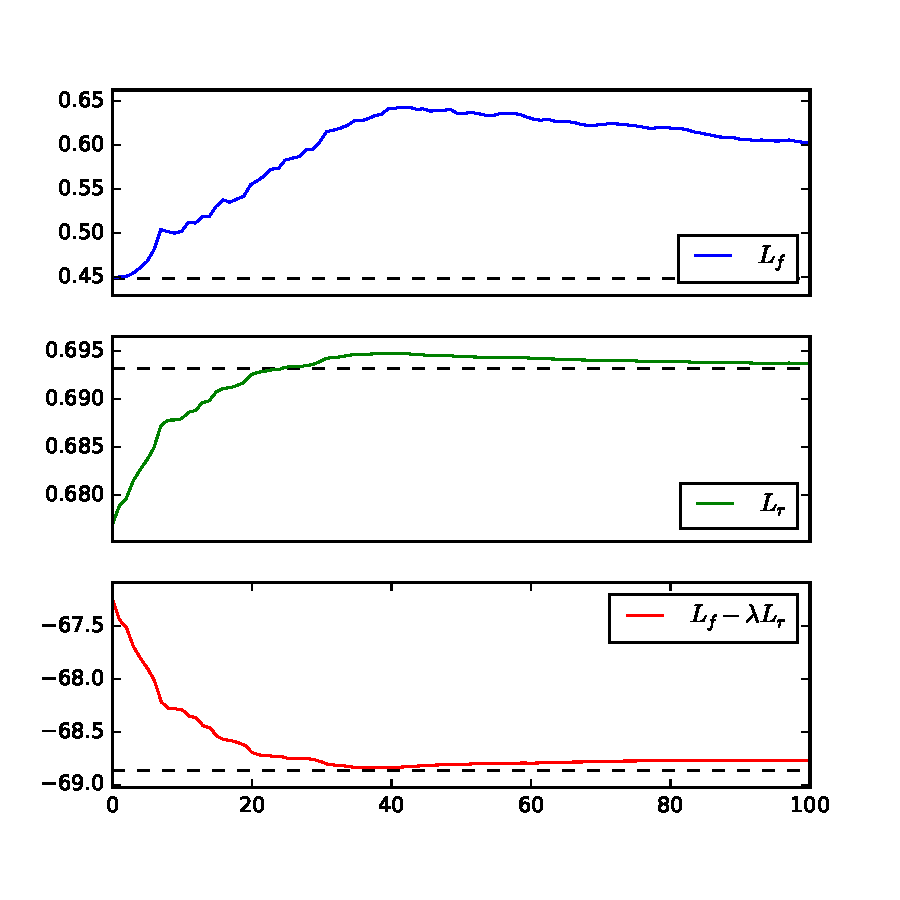
\includegraphics[width=0.48\textwidth]{figures/training.pdf}
    \vspace{-1cm}
    \caption{Toy example. Training curves for ${\cal L}_f(\theta_f)$, ${\cal L}_r(\theta_f, \theta_r)$
             and ${\cal L}_f(\theta_f) - \lambda {\cal L}_r(\theta_f, \theta_r)$.
             Adversarial training was performed for $200$ iterations, mini-batches of size $M=128$, $K=500$ and $\lambda=50$.}
    \label{fig:toy-training}
\end{figure}

As a guiding toy example, let us consider the binary classification of 2D
data drawn from multivariate gaussians with equal priors, such that
\begin{align}
    x &\sim {\cal N}((0,0), \begin{bmatrix}
                              1 & -0.5 \\
                              -0.5 & 1
                            \end{bmatrix}) &\text{ when } Y=0, \\
    x &\sim {\cal N}((1,1+Z),  \begin{bmatrix}
                              1 & 0 \\
                              0 & 1
                             \end{bmatrix}) &\text{ when } Y=1.
\end{align}
The continuous nuisance parameter $Z$ represents in this case our
uncertainty about the exact location of the mean of the second gaussian. Our goal is to
build a classifier $f(\cdot;\theta_f)$ for predicting $Y$ given $X$, but such that
the probability distribution of $f(X;\theta_f)$ is invariant with respect to the
nuisance parameter $Z$.

Assuming a gaussian prior $z \sim {\cal N}(0,1)$, we start by
generating training data $\{ x_i, y_i, z_i \}_{i=1}^N$, from which we train a
neural network classifier $f$ minimizing ${\cal L}_f(\theta_f)$ without
considering its adversary $r$. The network architecture comprises 2 dense hidden layers of 20
nodes with ReLU activations, followed  by a dense output layer with a single
node with a sigmoid activation. As shown in the upper plots of
Fig.~\ref{fig:toy}, the resulting classifier is not pivotal, as the
conditional probability densities of its decision scores $f(X;\theta_f)$ show
large discrepancies between values $z$ of the nuisance. While not shown here, a
classifier trained only from data generated at the nominal value $Z=0$ would
also not be pivotal.

Let us now consider the joint training of $f$ against an adversary $r$
implemented as a mixture density network modeling $Z|f(X;\theta_f)$ as a mixture
of five gaussians. As for $f$, the network architecture comprises 2 dense hidden
layers of 20 nodes with ReLU activations, but is followed by an output layer of
15 nodes corresponding to the means, standard deviations and mixture
coefficients of the five gaussians. Output nodes for the mean values come with
linear activations, output nodes for the standard deviations with exponential
activations to ensure positivity, while output nodes for the mixture coefficients
implement the softmax function to ensure positivity and normalization. When
running Algorithm~\ref{alg:adversarial-training} as initialized with the
classifier $f$ obtained previously, adversarial training effectively reshapes
the decision function so it that becomes almost independent on the nuisance
parameter, as shown in the lower plots of Fig.~\ref{fig:toy}. In particular,
the conditional probability densities of the decision scores $f(X;\theta_f)$ are
now very similar to each other, indicating only a small residual  dependency on the
nuisance, as theoretically expected. The dynamics of adversarial training is
illustrated in Fig.~\ref{fig:toy-training}, where the losses ${\cal L}_f$,
${\cal L}_r$ and ${\cal L}_f - \lambda {\cal L}_r$ are evaluated after each
iteration of Algorithm~\ref{alg:adversarial-training}. In the first iterations,
we observe that the global objective ${\cal L}_f - \lambda {\cal L}_r$ is
minimized by making the classifier less accurate, hence the corresponding
increase of ${\cal L}_f$, but which results in a classifier that is more
pivotal, hence the corresponding increase of ${\cal L}_r$ and the total net
benefit. As learning goes, minimizing $E$ then requires making predictions that
are more accurate, hence decreasing ${\cal L}_f$, or that are even less dependent on
$Z$, hence shaping $p_{\theta_r}$ towards the prior $p(z)$. Indeed, ${\cal L}_f$
eventually starts to slightly decrease, while remaining lower bounded by
$\min_{\theta_f} {\cal L}_f(\theta_f)$ as approximated by the dashed line in the
first plot. Similarly,  ${\cal L}_r$ tends towards the differential entropy
$H(Z)$ of the prior (where $H(Z) = \log(\sigma \sqrt{2 \pi e}) = 1.419$ in the
case of a gaussian with unit variance), as shown by the dashed line in the
second plot.
Finally, let us note that the ideal situation of a
classifier that is both optimal and pivotal appears to be unreachable for this
problem, as shown in the third plot by the  offset between ${\cal L}_f - \lambda
{\cal L}_r$ and the dashed line approximating $H({Y|X}) -
\lambda H(Z)$.

\subsection{High energy physics example}

Jets, or collimated sprays of particles produced by high energy quarks and
gluons, are produced ubiquitously at high energy colliders like the Large Hadron
Collider \citep{LHCMachine}.  In a wide array of new physics models, new highly
massive particles can decay though known heavy particles in Standard Model (SM),
like the $W$, $Z$, Higgs bosons, or top quarks which subsequently decay to
multiple quarks.  When these these heavy SM particles have significant energy,
the Lorentz boost causes their quark decay products to merge into a single jet
which has a rich internal substructure (see e.g.
\citep{Altheimer:2012mn,Altheimer:2013yza} and references therein).
Distinguishing these \textit{boosted jets} produced by heavy SM particles from
vanilla quarks and  gluons is a fundamental challenge in searching for signs of
new high mass particles. Challenging in it's own right, this classification
problem is made all the more difficult by the presence of pileup, or multiple
simultaneous proton-proton interactions occurring at the same time as the primary
interaction.  These pileup interactions produce additional particles that can
contribute significant energies to jets unrelated to the underlying
discriminating information. Thus pileup acts as a source of noise in the
classification problem.

The classification challenge used here is common in jet substructure
studies (see \citep{Khachatryan:2014vla,ATL-PHYS-PUB-2015-033,wbosonATLAS} and
references therein): we aim to discriminate between jets produced by quark or gluon fragmentation (the
background) and  boosted $W$ boson jets containing a collimated pair of
quarks (the signal).  We reuse the datasets used in reference
\citep{guest2016jet}.  Briefly summarizing, jets are built with the
anti-$k_T$ algorithm \citep{Cacciari:2008gp}
with radius parameter $R=1.2$, and trimmed \citep{Krohn:2009th} with subjets built with
the $k_T$ algorithm and parameter $f_{cut}=0.2$. The features used
in the classifiers are: trimmed jet invariant mass, N-subjettiness
$\tau_{21}^{\beta=1}$ \citep{nsub,Thaler2012}, and the energy correlation
functions \citep{Larkoski2013} $C_{2}^{\beta=1}$, $C_{2}^{\beta=2}$,
$D_{2}^{\beta=1}$, $D_{2}^{\beta=2}$.

As nuisance parameter, we consider events without pileup ($Z=0$) and
events with pileup ($Z=1$), for which an average number of $\langle \mu \rangle =
50$ unrelated additional pileup interactions are overlaid. Our goal is to build an accurate
classifier, for which we also want to minimize the effects due to the
uncertainties on the nuisance. More specifically, we choose to recast the
classification problem as a hypothesis test between signal+background (jets
originating from $W$ bosons or from quarks and gluons) and background
only (jets originating from quarks and gluons only) and tune the decision
threshold of our classifier by maximizing its approximate median significance
(AMS), when uncertainties in the background are taken into account (see Eqn.~20
of \citep{adam2014higgs}). Our motivation is that reducing the effects of
uncertainties by requiring independence of $Z$ with the classifier output $f(X;\theta_f)$ should
allow for a larger maximum significance.

To minimize the effects of $Z$ in the background events, we train a classifier
using  Algorithm~\ref{alg:adversarial-training} but consider the adversarial
term ${\cal L}_r$ conditioned on $Y=0$ only. Both $f$ and $r$ are neural
networks with 3 hidden layers of 64 nodes and ReLU activations, each terminated
by a single final output node with a sigmoid activation. Experiments are performed
on a subset of 150000 samples for training while AMS is evaluated on an independent test set of 5000000
samples. Both training and testing samples are weighted such
that the signal-to-background ratio is 1/10, allowing us to probe the
efficacy of the method proposed here in a background dominated
environment. Results reported below are averages over 5 runs.

\begin{figure}
    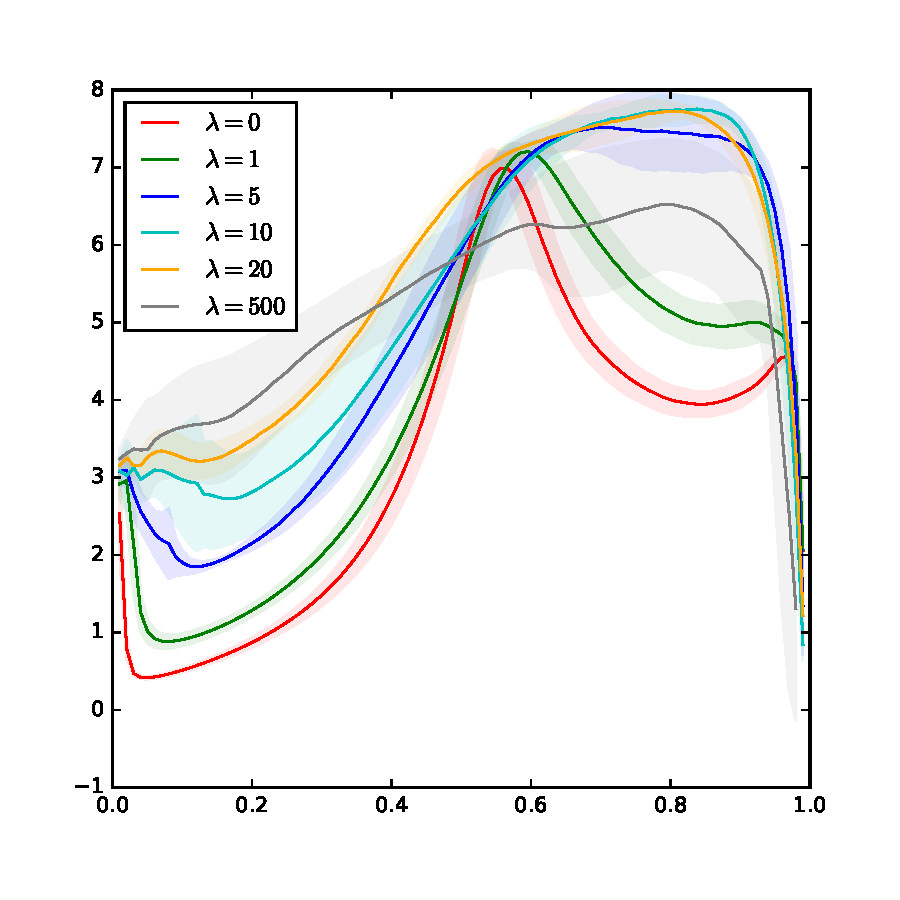
\includegraphics[width=0.48\textwidth]{figures/ams.pdf}
    \vspace{-1cm}
    \caption{Approximate median significance as a function of the decision threshold
             on the output of $f$.  As shown at $\lambda=10$, trading
             classification accuracy for independence with respect to pileup
             results in a positive total net benefit in terms of statistical significance.}
    \label{fig:physics-ams}
\end{figure}

As  Fig.~\ref{fig:physics-ams} illustrates, without adversarial training (at
$\lambda=0$), the maximum significance peaks at $7$. By contrast, as the
independence constraint is made stronger (for $\lambda > 0$) the AMS peak moves
higher, with a maximum value around  $7.8$ for $\lambda=10$. In other words,
trading classification accuracy for independence with respect to pileup results
in a positive total net benefit in terms of statistical significance. Setting
$\lambda$ too high however (e.g. $\lambda=500$) results in a decrease of the
maximum significance, by focusing the capacity of $f$ too strongly on
independence, at the expense of classification accuracy. As demonstrated in this
example, controlling the classification versus pivot trade-off through $\lambda$
therefore gives us a principled and effective approach for maximizing
significance by desensitizing the classifier output $f(X;\theta_f)$ in the most
beneficial way.


% ==============================================================================

\section{Related work}

To account for systematic uncertainties, experimentalists in high energy physics
typically take as fixed a classifier $f$ built from training data for a nominal
value $z_0$ of the nuisance parameter, and then propagate uncertainty
 by estimating $p(f(x)|z)$ with a parameterized calibration
procedure. Clearly, this classifier is however not optimal for $z \neq z_0$.
To overcome this issue, the classifier $f$ is sometimes built instead on a mixture
of training data generated from several nominal values $z_0, z_1, \dots$ of the nuisance.
While this certainly improves with respect to classification performance,
there is however no guarantee that the resulting classifier is pivotal, as shown
previously in Section~\ref{sec:toy}.
As an alternative, parameterized
classifiers~\citep{cranmer2015approximating,Baldi:2016fzo} directly take
(nuisance) parameters as additional input variables, hence ultimately providing
the most statistically powerful approach for incorporating the effect of
systematics on the underlying classification task.  As argued in
\citep{Neal:2007zz}, such classifiers can however not be used on real data since
the correct value $z$ of the nuisance often remains unknown. This is typically
not an issue in the context of parameter
inference~\citep{cranmer2015approximating}, where nuisance parameters are
marginalized out, but otherwise often limits the range of their applications. In
practice, parameterized classifiers  are also computationally expensive to build
and evaluate. In particular, calibrating their decision function, i.e.
approximating $p(f(x,z)|z)$ as a continuous function of $z$, remains an open
challenge. By contrast, constraining $f$ to be pivotal yields a classifier which
may not be optimal with respect to $Y|X,Z$, as discussed in
Section~\ref{sec:theory}, but that can otherwise be used in a wider range of
applications, since knowing the correct value $z$ of the nuisance is not
necessary. Similarly, calibration needs to be carried out only once, since  the
dependence on the nuisance is now built-in.

In machine learning, learning a pivotal quantity can be related to the problem
of domain adaptation
\citep{blitzer2006domain,pan2011domain,gopalan2011domain,gong2013connecting,baktashmotlagh2013unsupervised,ganin2014unsupervised},
where the goal is often stated as trying to learn a domain-invariant
representation of the data. Likewise, our method also relates to the problem of
enforcing fairness in classification \citep{zemel2013learning,feldman2015certifying,EdwardsS15,zafar2015fairness}, which
is stated as learning a classifier that is independent of some chosen attribute
such as gender, color or age. For both families of methods, the problem can
equivalently be stated as learning a classifier which is a pivotal quantity with
respect to either the domain or the selected feature. In this context,
\citep{ganin2014unsupervised,EdwardsS15} are certainly among the closest to our
work, in which domain invariance and fairness are enforced through an
adversarial minimax setup composed of a classifier and an adversary
discriminator. Following this line of work, our method can be regarded as a
generalization that also supports the continuous case, which can be viewed as
handling infinitely many domains, provided they can be continuously
parameterized, or as enforcing fairness over continuous attributes.


% ==============================================================================

\section{Conclusions}


% ==============================================================================

\begin{acknowledgments}
\end{acknowledgments}


% ==============================================================================

\bibliographystyle{acm}
\bibliography{bibliography.bib}

\end{document}
